% Chapter 1

\chapter{Driving signals} % Main chapter title
\label{Ch:signals} % For referencing the chapter elsewhere, use \ref{Chapter1} 

Complex networks grow by adding new nodes, and growing network models consider growth constant over time. This approximation is sufficient for explaining how properties of complex networks can emerge; for example, we find scaling of degree distribution in the Barabasi-Albert model. Models mainly focus on linking rules and their influence on the topology of complex networks. 

Still, the growth of real systems changes over time. In online social networks, new users join daily, and the users' activity might have bursty nature. We can consider a co-authorship network, where links are created between scientists when they publish a paper. The dynamic of real networks can be complex and highly influenced by nonlinear signals. The growth signal, the number of new nodes in each time step, has cycles and trends. Circadian cycles are directly reflected in growth signals, and we also find long-range correlations and multifractal properties. 

In this chapter, we explain the properties of growth signals, both real and computer-generated. We analyze networks created with a growing network model where the interplay between ageing and preferential attachment shapes their structure. We are interested in incorporating non-constant growth signals into the model and measuring their impact on complex networks. Differences between networks with the same number of nodes and links can be observed by analyzing connectivity patterns. Figure \ref{fig:ciljevi} summarizes our goals. 

\begin{figure}[!ht]
	\centering
	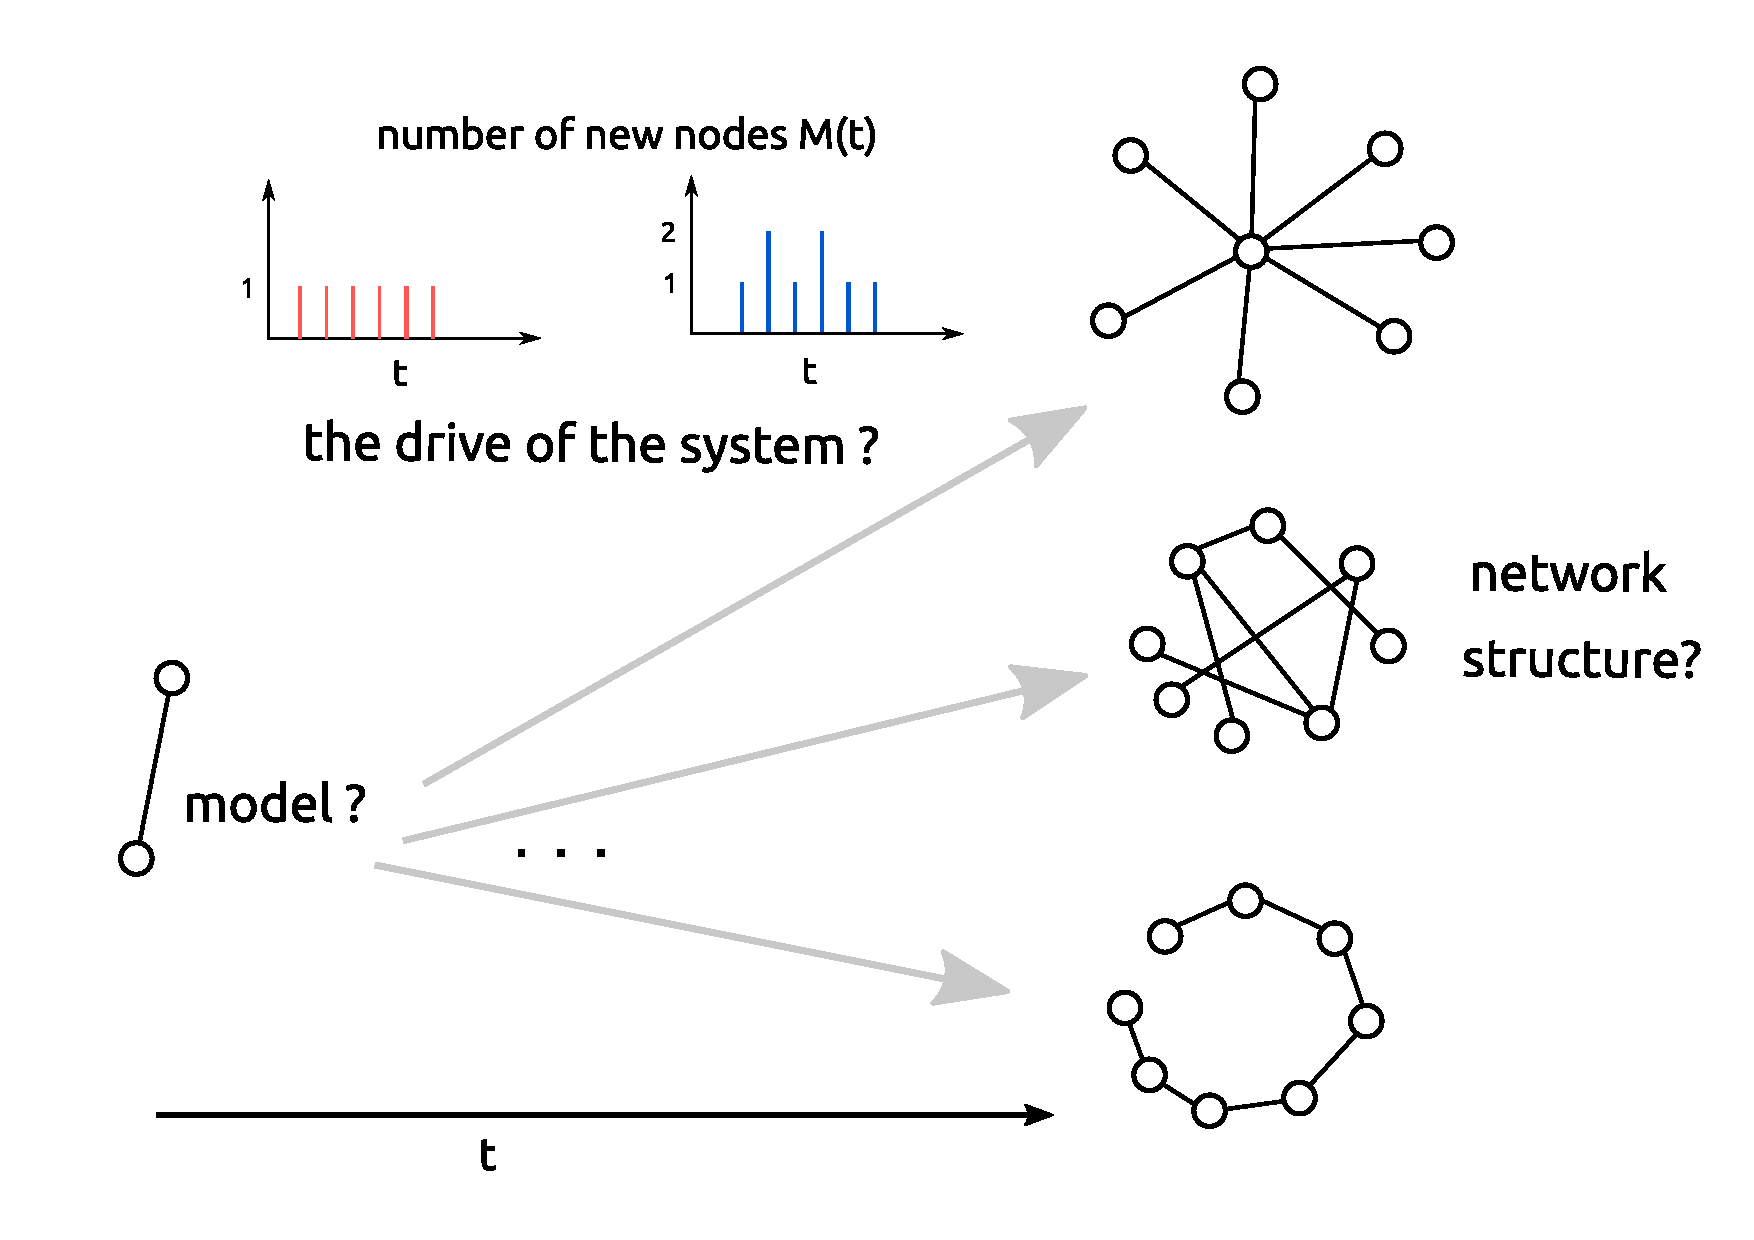
\includegraphics[width=0.7\linewidth]{chapter3/ciljevi.pdf}
	\caption[Nonlinear growth of the network.]{The open question is how nonlinear signals, in combination with the network model, influence the network's structure. Under what circumstances do networks have the scale-free, hub-spoke or chain structure? }
	\label{fig:ciljevi}
\end{figure}

\section{Aging network model with growth signal}

To enable nonlinear network growth in the number of nodes, we need to adapt the existing models such that at each time step, we can add $M\geq1$ new nodes that make $L\geq1$ links with existing nodes in the network. The master equation $N_k$, $k$ degree nodes can be written as: 

\begin{equation}
\partial_{t}N_{k}=\sum^{M(t)}_{j=1}r_{k-j\longrightarrow k}N_{k-j}-\sum^{M(t)}_{j=1}r_{k\longrightarrow k+j}N_{k}+M(t)\delta_{k,L} . \label{eq:aging_master}  
\end{equation}

We add $M(t)$ nodes with $L$ links at each time step. As multiple links between two nodes are not allowed, we'll get $M(t)$ new nodes with degree $L$, which describes the third term in the equation. Old nodes can increase their degree from 1 to $M(t)$, as different new nodes can choose the same node. The first term in the equation describes nodes with degree $k\in\{k-M(t),\ldots, k-1\}$ that getting degree $k$, while in second term nodes with degree $k$ entering degree  $k\in\{k+1,\ldots, k+M(t)\}$. The quantities $r_{k-j\longrightarrow k}$ and $r_{k\longrightarrow k+j}$ are the rates that express the transitions of a node from class with degree $k-j$ to one with degree $k$ and from class with degree $k$ to class with degree $k+j$ respectively.  

For the model, we choose the aging model where linking probability depends on network degree $k$ and its age $\tau$, $\Pi_{i}(t)\sim k_{i}(t)^{\beta}\tau_{i}^{\alpha}$. With this linking probability, the master equation was solved for $M(t)=const.=1$, using approach \cite{dorogovtsev2001b}. When $M(t)$ is the correlated function, the equation is not solvable analytically. Instead, we use numerical simulations to study the influence of the signal $M(t)$ on the network structure. When we add only one link per node $L=1$, networks are uncorrelated trees. To obtain the clustered structures, we need to use $L>1$; each new node can create more than one link. Finally, we focus on the aging model parameters $-\infty<\alpha\leq-1$ and $\beta\geq1$. We expect a critical line $\beta(\alpha^{*})$ where scale-free networks can be found. Under critical line, networks have stretched exponential degree distribution, and for large $\beta$ small-world networks are present. 

Finally, we need to define the new nodes' time series. We focus on the growth of two real systems, the \textbf{TECH} \cite{smiljanic2017associative} community in the Meetup website and on two months of \textbf{MySpace} \cite{suvakov2013} social network. 

\subsection{Time-series from real systems}

MySpace signal is the number of new members who appear for the first time in the data. Here, the time step is one minute. The MySpace signal has $T = 3162$ steps, with  $N = 10000$ members. To describe the properties of the signal, we use Multifractal detrended analysis and calculate the Hurst exponent on different scales, showing the right pane of the Figure, \ref{fig:myspace_signals}. It is multifractal $q<0$ and becomes constant for $q>0$; it has long-range correlations as $H(q=2)=0.6$. My Space signal has cycles characteristic of the human circadian rhythm, Figure $\ref{fig:myspace_signals}$. We can easily destroy trends and cycles if we randomize the MySpace signal. The randomization is done with the reshuffling procedure, where we keep number where we keep the number of nodes, length and the mean value of the signal. The inset of the original and randomized signals show the time series' global profile; we find that trends are destroyed. Also, the randomized MySpace signal no longer has long-range correlations; the Hurst exponent indicates short-range correlations $H=0.5$, and the signal becomes monofractal.    


\begin{figure}[H]
	\centering
	\begin{minipage}[b]{0.4\textwidth}
		\centering
		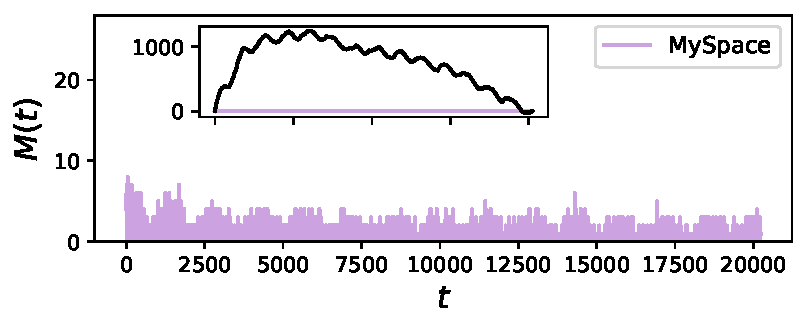
\includegraphics[width=\textwidth]{chapter3/signal4.pdf}\\
		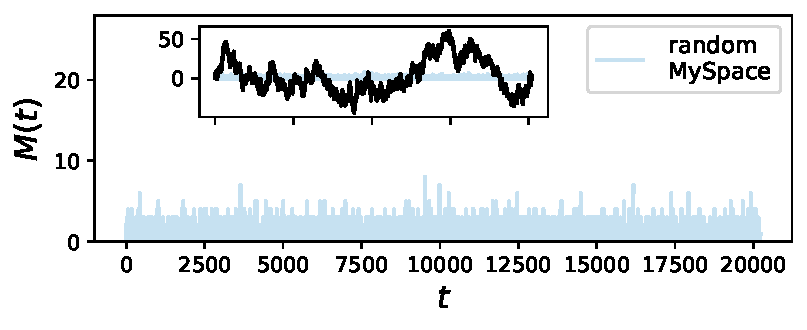
\includegraphics[width=\textwidth]{chapter3/signal5.pdf}
	\end{minipage}
	\begin{minipage}[b]{0.45\textwidth}
		\centering
		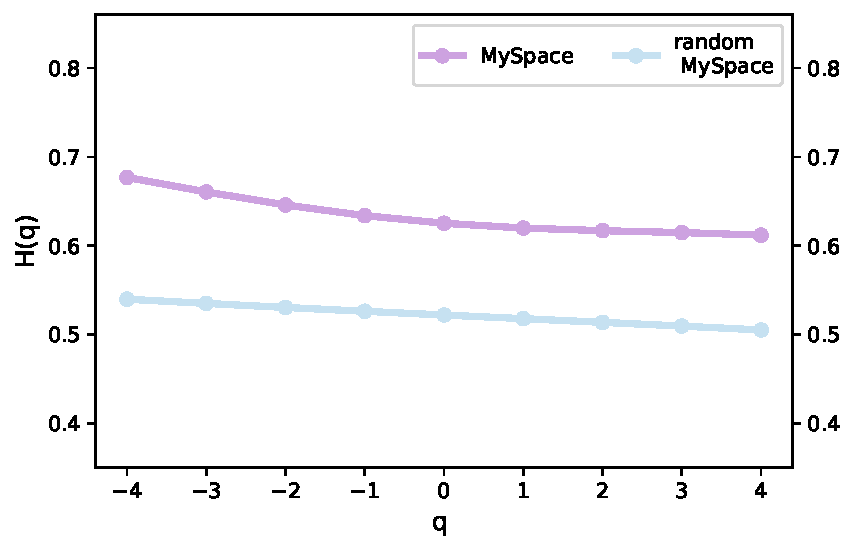
\includegraphics[width=\textwidth]{chapter3/hurst_myspace.pdf}
		\vspace{0.01cm}
	\end{minipage}
	\caption[Properties of MySpace signal.]{MySpace signal, the random MySpace signal (left pane) and the dependence of multifractal Hurst exponent $H(q)$ of the scale $q$. (right pane)}
	\label{fig:myspace_signals}
\end{figure}

\begin{figure}[ht]
	\centering
	\begin{minipage}[b]{0.4\textwidth}
		\centering
		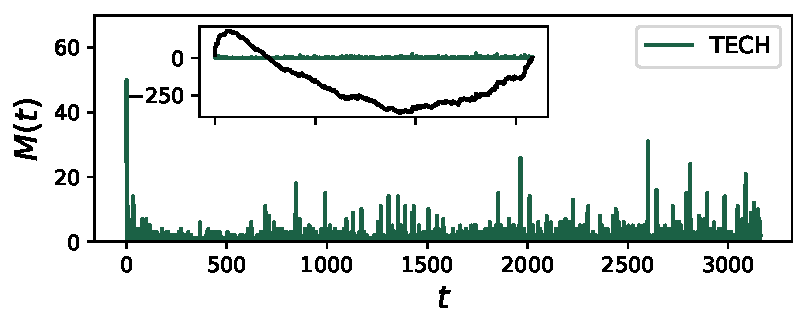
\includegraphics[width=\textwidth]{chapter3/signal1.pdf}\\
		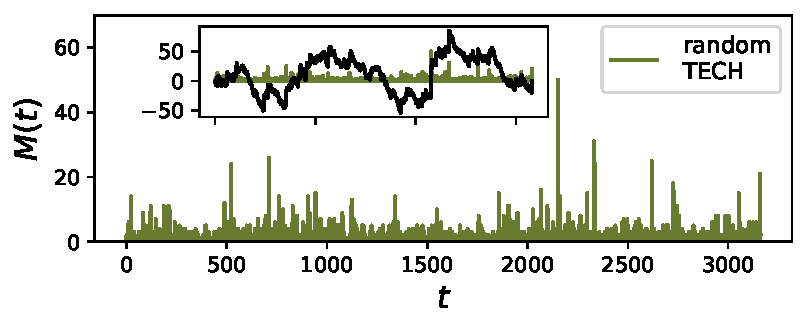
\includegraphics[width=\textwidth]{chapter3/signal2.pdf}\\
		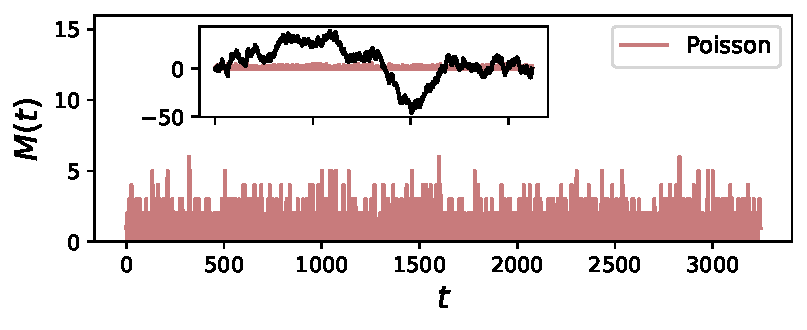
\includegraphics[width=\textwidth]{chapter3/signal3.pdf}
		
	\end{minipage}
	\begin{minipage}[b]{0.45\textwidth}
		\centering
		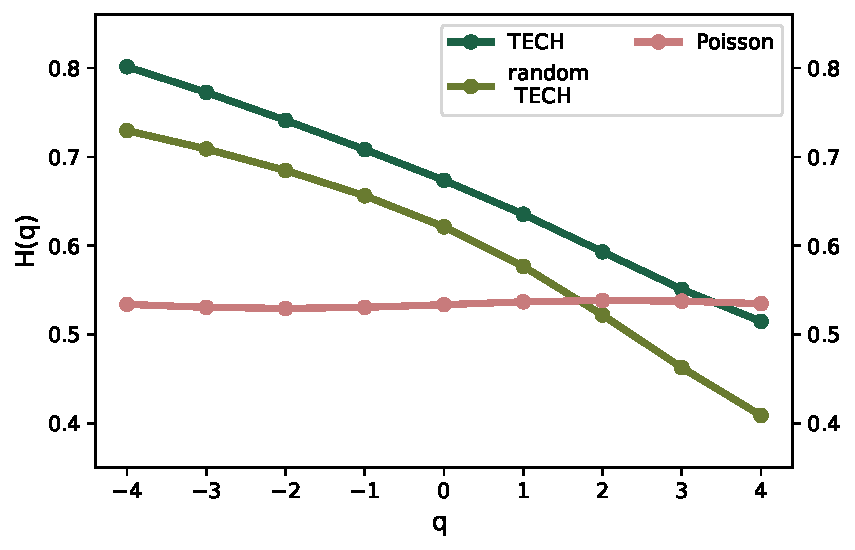
\includegraphics[width=\textwidth]{chapter3/hurst_tech_1.pdf}
		\vspace{1cm}
	\end{minipage}
	\caption[Properties of the TECH and Poisson signals.]{TECH signal, the random TECH signal (left pane) and the dependence of multifractal Hurst exponent $H(q)$ of the scale $q$. (right pane)}
	\label{fig:tech_signals}
\end{figure}

The TECH is a group from the Meetup website that gathers users interested in technology. Using the Meetup website, they organize offline events. The time unit in this time series is an event since then are created links between events. The TECH time series $M(t)$ represents the number of users who joined the TECH community and visited the event for the first time. The time series length is $T=3162$ steps, and we count $N=3217$ members in the TECH community for a given period, Figure \ref{fig:tech_signals}. TECH signal has long-range correlations with Hurst exponent $H(q=2)=0.6$. Also, we find that TECH is multifractal, as the Hurst exponent is not constant across the scales. The multifractality originates not only from signal trends but also from the broad probability distribution of time series. If we randomize the TECH signal, we can easily destroy trends and cycles, but the signal keeps multifractal properties, meaning that broad probability distribution can not be eliminated. Therefore, we generate the uncorrelated signal from the Poissonian probability distribution. The length of this signal is  $T = 3246$, while we keep the number of nodes $N$ the same as in the TECH signal.


\subsection{D-measure}

We can compare the networks with the same number of nodes and links generated with growth signals with different properties. We use a growing network model where we vary parameters $-3<\alpha\leq-1$ and $-3\leq\beta\leq1$. We also vary the network density, $L\in\{1,2,3\}$. For each set of model parameters $\alpha, \beta, L$ and each signal $M(t)$, we create the sample of $100$ networks. Besides this, for the same set of parameters, we generate the sample of networks with $N=10000$ and $N=3217$ nodes grown with constant signal $M(t)=1$; one node is added to the network at each time step. To examine how different growing signals influence the structure of networks, we use D-measure \cite{tiago2}, defined methodology chapter. We equally consider the global and local properties, setting parameter $w=0.5$. We compare the networks grown with the constant and fluctuating signal with D-measure for all network pairs between two samples and average the result. The advantage this measure has is that it can measure the distance between two network structures, even if they are generated with the same model; that was not the case with Hamming distance or graph editing distance \cite{tiago2}.

Figure \ref{fig:dmeasure} presents the results for D-measure. The most significant distance between networks is along the critical line $\beta(\alpha^{*})$ of the aging model. The fluctuations present in the signal mainly influence the scale-free networks. Structural differences exist for networks away from this line, but they are much smaller. The D-measure is close to zero for gel small-world networks, $\beta>\beta^{*}$. Under critical line, $\beta<\beta^{*}$, the D-measure depends on the properties of the signal. If we fix network density $L$, the position of the critical line is independent of the properties of the signal. Still, with higher link density, the critical line slightly moves toward larger $\beta$; see Figure \ref{fig:dmeasure}.

\begin{figure}[ht]
	\centering
	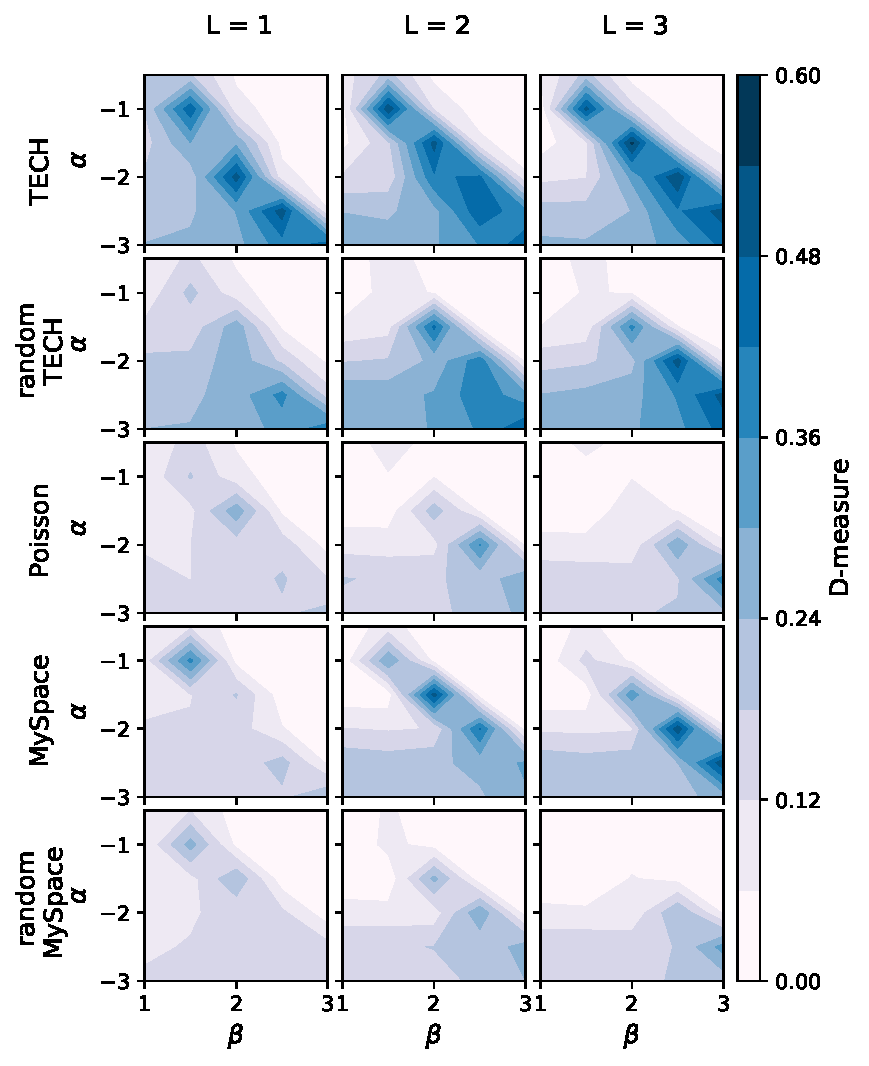
\includegraphics[width=0.6\linewidth]{chapter3/Ddistance.pdf}
	\caption[D-measure for networks generated with real signals.]{The comparison of networks grown with growth signals shown in figures \ref{fig:tech_signals} and \ref{fig:myspace_signals} versus ones grown with constant signal $M=1$, for the value of parameter $\alpha\in[-3,-1]$ and $\beta\in[1,3]$. $M(t)$ is the number of new nodes, and $L$ is the number of links added to the network in each time step. The compared networks are of the same size.}
	\label{fig:dmeasure}
\end{figure}

In the region around the critical line, we find that the D-measure depends on the properties of the signal. Multifractal signals TECH has the most considerable impact on network structure; the maximum value of the D-measure is $D_{max}=0.552$. Similar behaviour is discovered for other multifractal signals, random TECH and MySpace. The difference exists for networks generated with uncorrelated signals: random MySpace and Poisson, but it is much smaller.

D-measure rises for lower $\alpha$. In the case of a constant signal, the number of nodes added to the network is equal for each time step, so at time interval $T$, the network has $MT$ nodes. In fluctuating signal, the number of nodes added during time interval $T$ vary. Hubs emerge faster in signals, such as TECH, where there are peaks in the number of new users. As we decrease the parameter $\alpha$, fluctuations in the signal become more critical, and the hubs emerge even for uncorrelated signals. The trends in the real signals further promote the emergence of hubs in the network.  

\subsection{The structure of networks}

We examine degree distribution, degree correlations and clustering coefficient of networks generated by real signals. These measures have provided a sufficient set for describing the structure of complex networks. Results showed that multifractals influence networks more than monofractals; it is most prominent in scale-free networks. 

Figure \ref{fig:properties_net} shows properties of networks generated with model parameters $L=2$, $\alpha=-1.0$, $\beta=1.5$, that lie on the critical line. The degree distributions $P(k)$ of networks generated with real signals TECH and MySpace have super-hubs emerged. Degree distributions generated with randomized and white noise signals do not differ from the degree distribution of networks generated with the constant signal. Networks generated with real signals average neighbouring degree $\langle k\rangle_{nn}(k)$ and clustering coefficient $c(k)$ depend on node degree. In contrast, networks generated with constant and randomized signals weakly depend on the degree $k$.

We also find structural differences between networks, obtained with model parameters under the critical line $\alpha<\alpha^{*}$, see Figure \ref{fig:properties_net}. The difference is mainly found in the TECH signal. Degree distribution $P(k)$ shows the emergence of hubs in networks grown with TECH signal, while the randomized and Poisson signals are more similar to networks grown with the constant signal. MySpace signal, whose generalized Hurst exponent $H(q)$ weakly depends on scale parameter $q$ and whose long-range correlations and trends are easily destroyed, do not influence the structure of networks more than constant or randomized signal.   

The properties of the time-varying signal do not influence the topological properties of small-world gel networks, Figure \ref{fig:properties_net}. Here model promotes the existence of hubs. As this is the mechanism through which the fluctuations alter the structure of evolving networks, the properties of the signal are not relevant.   

\begin{figure}[H]
	\centering
	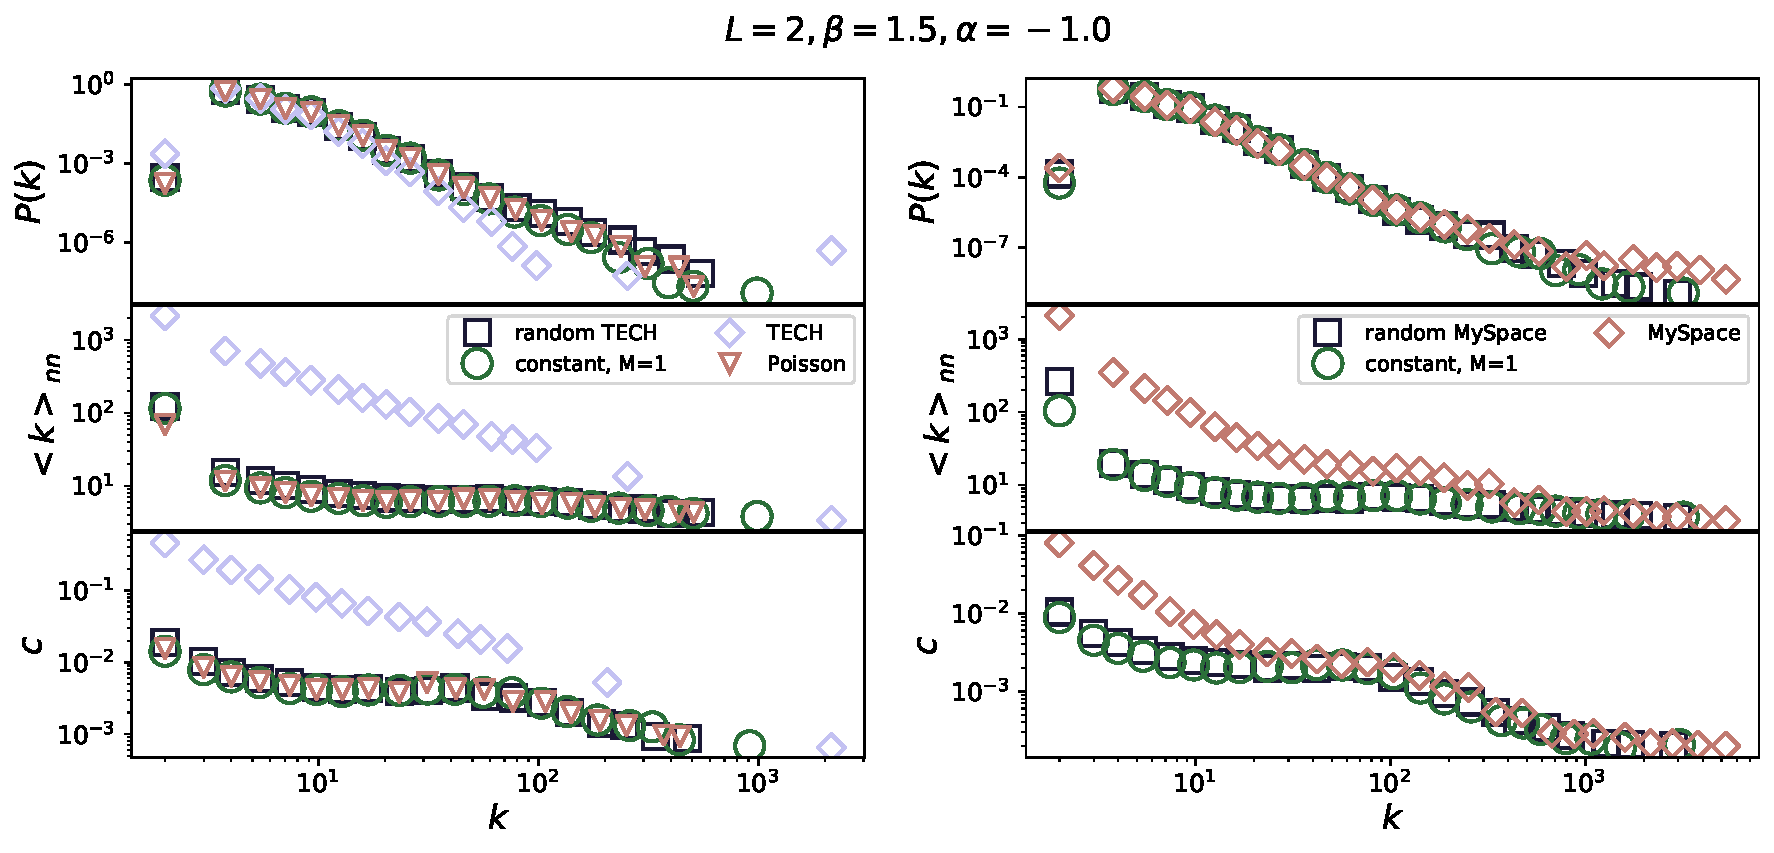
\includegraphics[width=0.9\textwidth]{chapter3/b1.pdf}
	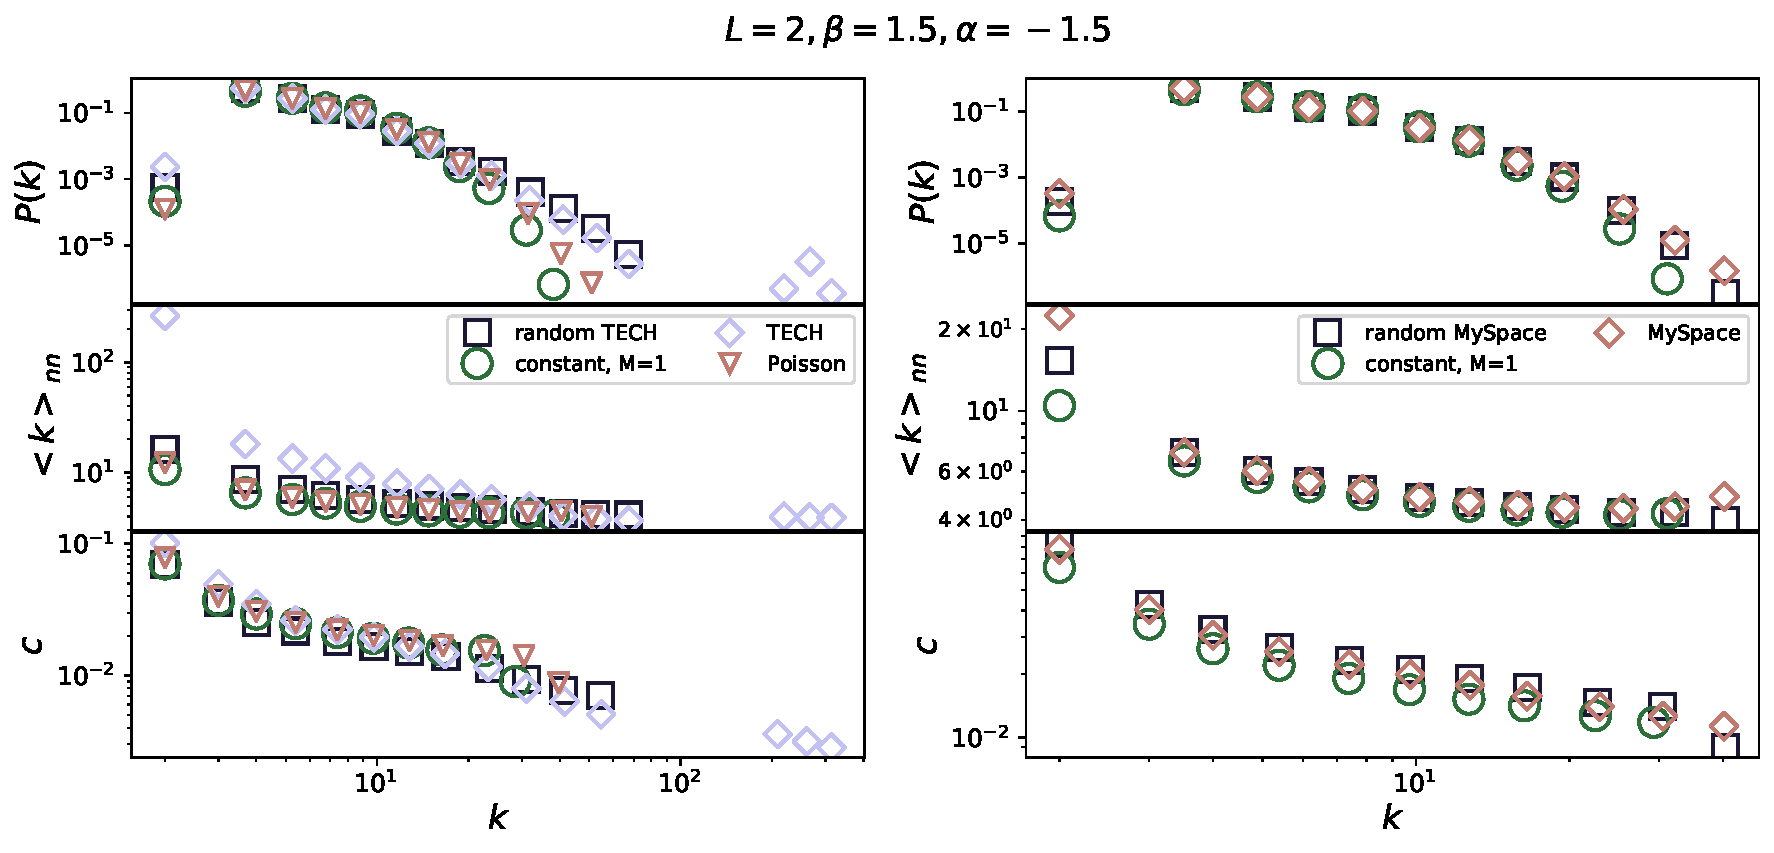
\includegraphics[width=0.9\textwidth]{chapter3/b3.pdf}
	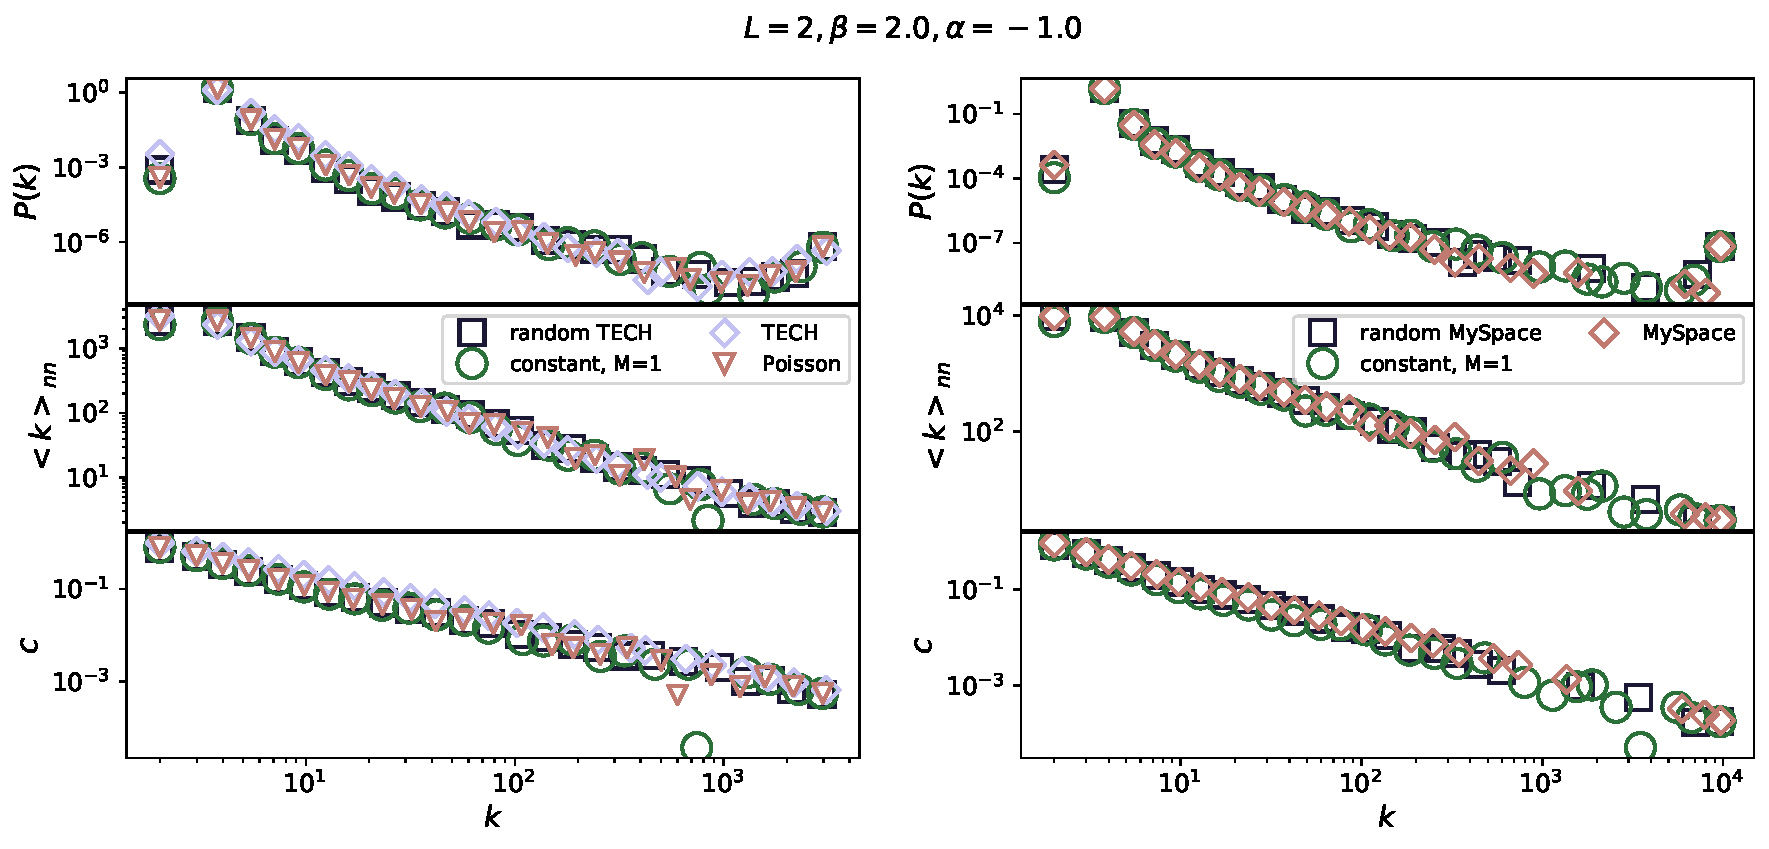
\includegraphics[width=0.9\textwidth]{chapter3/b2.pdf}
	\caption[Structural properties of networks.]{Degree distribution, the dependence of average first neighbour degree on node degree, dependence of node clustering on node degree for networks grown with different time-varying and constant signals. Model parameters have value $\alpha=-1.0$, $\beta=1.5$  and $L=2$ for all networks. The networks are from the scale-free class. Model parameters have value $L=2, \alpha=-1.5$, $\beta=1.5$. The networks have stretched exponential degree distribution. Model parameters have value $ L=2, \alpha=-1.0$, $\beta=2.0$. Generated networks have small-world properties.}
	\label{fig:properties_net}
\end{figure}

\section{Long range correlated signals}

The previous section showed that the growth signal of real systems has complex dynamics. Besides long-range correlations, we also find multifractal properties, and it is hard to isolate individual effects and analyze their influence separately. When this is the case, synthetic signals with specific characteristics can help to verify our findings in real systems. The long-range correlated properties can be included in time series using Fourier filtering transform method \cite{makse1996method}. 

The long range correlated data have power-law correlations $C(s)= <x_i x_{i+s}> = s ^ {-\gamma}$ characterized with coefficient $\gamma$. Hurst exponent depends on $\gamma$ as  $H = 1- \frac{\gamma}{2}$. The Fourier transform gives us the power spectrum of the time series $S(f)$, which is a function of the frequency $f$. For the long-range correlated data, it depends on coefficient $\beta = 1-\gamma$ and has the form:
\begin{equation}
S(f) \sim f^{-\beta}
\end{equation}
We can generate the data using Fourier filtering with $\beta = 2H - 1$, as following:

\begin{itemize}
	\item first generate one-dimensional sequence of uncorrelated random numbers $u_i$ from Gaussian distribution with $\sigma=1$.
	\item calculate the Fourier transform of the generated sequence, $u_q$, the spectrum is flat as data correspond to white noise.
	\item then filter the power spectrum with $f^{-\beta/2}$, so the function will follow the power spectrum expected for data with long-range correlations. 	
	\item  calculate the inverse Fourier transform $x_i$. It converts data to the time domain where the signal has desired long-range correlations.
	
\end{itemize}     

The Fourier filtering method generates the Gaussian distributed data, so data are without broad distributions, nonlinear or multifractal properties. Using this method, we generated the signals for different values of the Hurst exponent; see Figure \ref{fig:monofractals}. The obtained signals are round to integers, and the mean values of signals are close to $4$.

\begin{figure}[ht!]
	\centering
	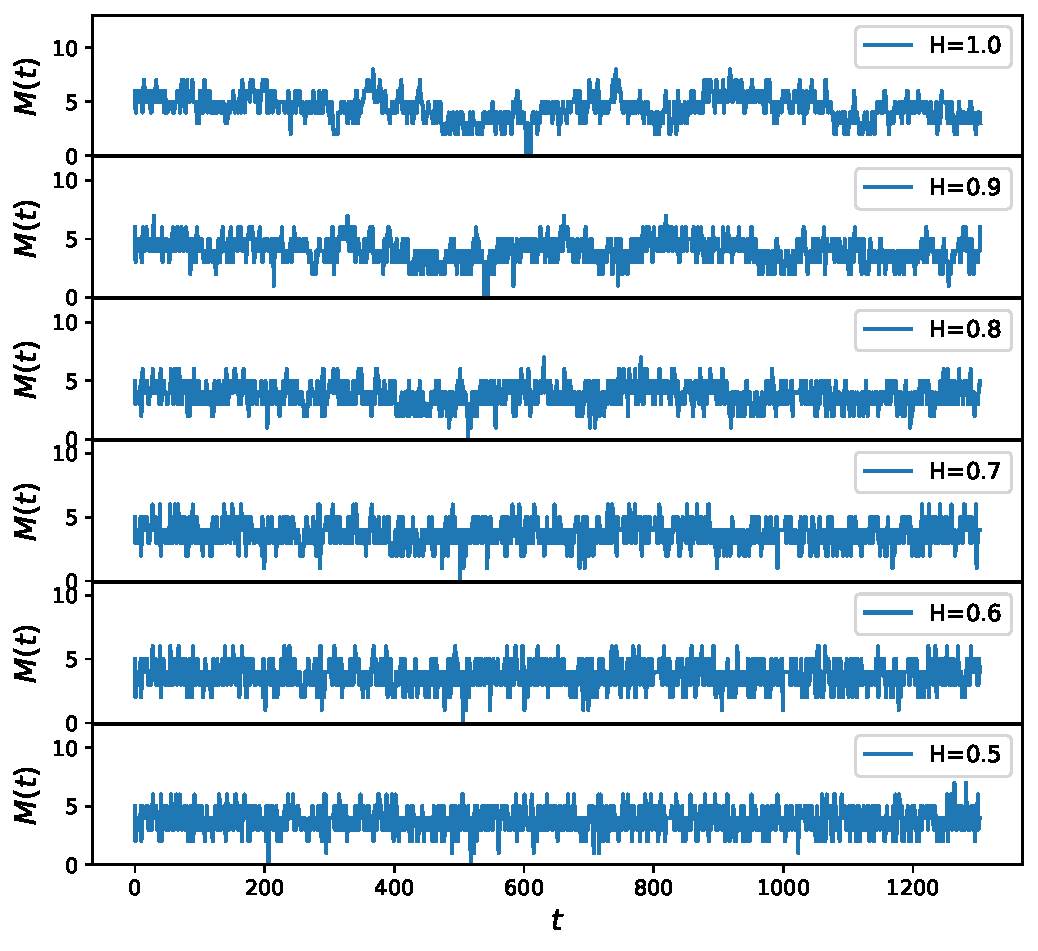
\includegraphics[width=0.6\linewidth]{chapter3/monofractals.pdf}
	\caption[Long range correlated monofractal signals]{Monofractal signals generated with Fourier filtering method for different Hurst exponents}
	\label{fig:monofractals}
\end{figure}  


As before, we focus on the region of the model phase diagram with negative $\alpha$ and positive $\beta$ as the transition line from stretched-exponential across scale-free to the small world-gel networks are found. We take a range of parameters  $-3\leq\alpha\leq-0.5$ and $1\leq\beta\leq3$ with steps $0.5$, and we also vary the number of links each new node can create $L\in{1, 2, 3}$. For each combination of $(\alpha, \beta, L)$, we generate the sample of $100$ networks and compare the structure of the network grown with fluctuating signals with different Hurst exponent $H \in \{0.5, 0.6, 0.7, 0.8, 0.9, 1.0\}$ and constant signal $M=4$. The results represented by D-measure, shown in Figure \ref{fig:Ddist_m}, are obtained by averaging the D-measure between all possible pairs of generated networks.   

The higher values of the D-measure are found in the region of critical line $\beta(\alpha^{*})$. The most considerable influence is on networks with the scale-free distribution. Comparing D-distance in only one point of the phase diagram, for example, $L=1, \alpha = -2.5, \beta = 2.5$, we find that when the Hurst exponent is more prominent, correlations in the signal make a bigger impact on the network structure. D-measure between networks grown by signal with Hurst exponent $H=1.0$ and the constant signal is $D(H=1.0, M=4) = 0.405$, while between networks grown with a signal with $H=0.8$ and the constant signal is $D(H=0.8, M=4) = 0.316$. For $\alpha>\alpha^{*}$, networks have similar structural properties, and D-measure is close to 0. In the region of networks with stretched exponential degree distribution, $\alpha<\alpha^{*}$  differences are small. 

\begin{figure}[H]
	\centering
	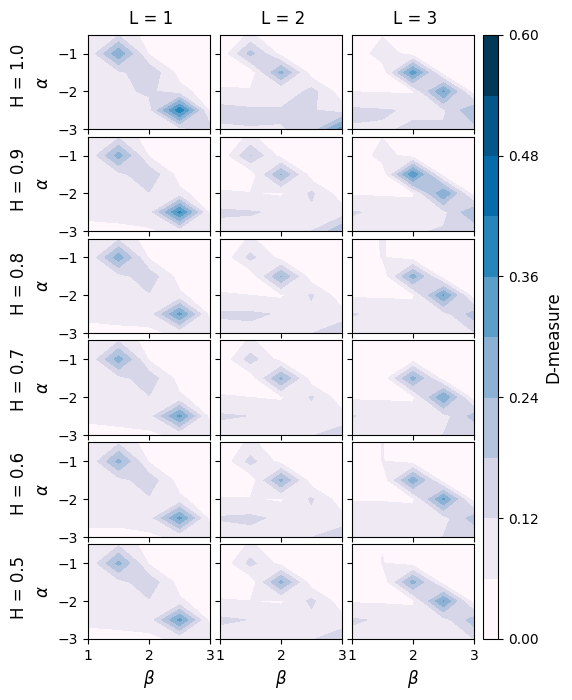
\includegraphics[width=0.6\textwidth]{chapter3/Ddist_M4_w10.5_w20.5.png}
	\caption[D-distance for networks generated with monofractal signals. ]{D-distance between networks generated with different long-range correlated signals with a fixed value of Hurst exponent and networks generated with constant signal M=4.}
	\label{fig:Ddist_m}
\end{figure}


We further explore the assortativity index and clustering coefficient of generated networks. Figure \ref{fig:aindex} are results for several ageing model parameters that show the difference between networks this model can produce. All networks are disassortative, with a negative degree-degree correlation index. For the parameters below critical line values, $\alpha=-2.5, \beta=1.5$ $r$ does not depend on the Hurst exponent. Above the critical line are small-world networks, and they are disassortative. The minimum value of the assortativity index is $r =-1$, for $L=1$, indicating the presence of hubs connecting many nodes. The assortativity index grows slightly with link density. 

In the region of critical parameters, the assortativity index depends on the value of the Hurst exponent. Signals With Hurst exponent $H>0.8$ have a larger influence on the assortativity index. Networks become more disassortative; see the line for parameters $L=1, \alpha=-2.5, \beta=2.5$ in Figure \ref{fig:aindex}. The long-range correlations have a stronger effect on the evolution of networks with lower density. 

\begin{figure}[h!]
	\centering
	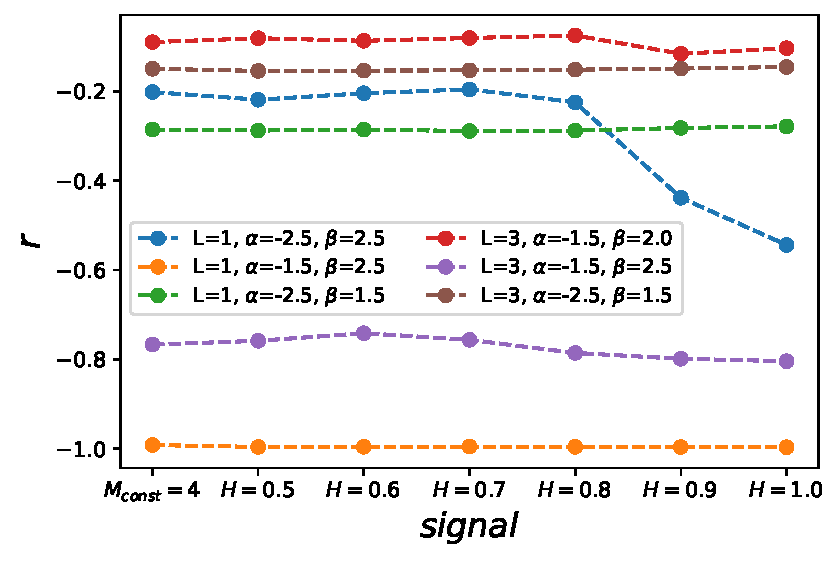
\includegraphics[width=0.45\textwidth]{chapter3/aindex.pdf}
	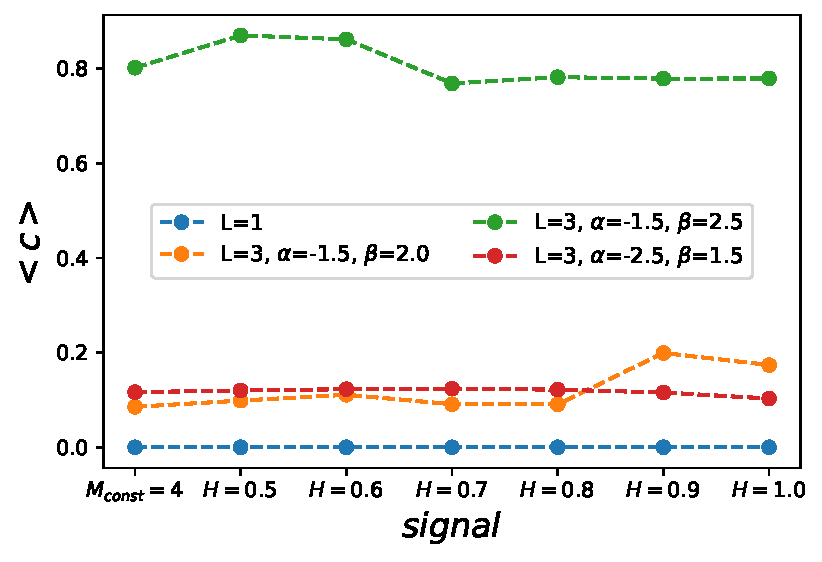
\includegraphics[width=0.45\textwidth]{chapter3/clustering.pdf}
	\caption[Assortativity index and mean clustering coefficient.]{Mean assortativity index for networks generated  with different model parameters $\alpha, \beta, L$ and different long-range correlated signals with Hurst exponent $H$.}
	\label{fig:aindex}
\end{figure} 

Figure \ref{fig:aindex} shows the mean clustering coefficient. For $L=1$, networks are uncorrelated trees with clustering coefficient $0$. For network density $L>1$, nodes are organized into clusters. Under the critical line, for parameter $L=3, \alpha=-2.5, \beta=1.5 $, the clustering coefficient is constant and low. Similar values are obtained for the clustering coefficient for critical parameters $L=3, \alpha=-1.5, \beta=2.0$, but for Hurst exponent $H>0.8$ clustering coefficient increases. Small world networks,  $L=3, \alpha=-1.5, \beta=2.5$ are clustered, the value of $<c>$ is high.  The value of clustering for networks created with the constant signal is 0.8. Networks grown with white noise signal and signal with H=0.6 have higher clustering values, while networks grown with signals with a Hurst exponent larger than 0.6 have the same clustering value below 0.8. 

\section{Conclusions}

In this chapter, we focused on the properties of growth signals and their influence on the system. The network grows at a constant rate in the simplest complex network models. In reality, growth signals are not constant, they are temporally correlated, and the main question is what impact they have on the complex networks. We combined the ageing model with nonlinear growth while we used real and computer-generated long-range correlated signals for growing signals. The network structure depends on the type of signals.

The ageing model can generate different complex networks depending on the model parameters. Our results showed that the most significant difference between networks generated with a constant and fluctuating signal is found on the critical line, where networks have broad degree distribution. While temporal correlations do not affect the degree distribution, the networks generated with fluctuating signals are more clustered and have more significant degree-degree correlations. The D-measure indicates that structural differences exist even for networks generated with white noise. For multifractal signals, we find the larger values of the D-measure. Furthermore, if we focus only on monofractal signals, characterized by the fixed value of Hurst exponent, $H$, the difference between networks rises with $H$. 

Away from the critical line, the fluctuations do not strongly influence the network structure; D-measure is close to zero. In small-world networks, super-hubs emerge, and no matter how strong correlations, trends or cycles exist in the signal, the structure of small-world networks does not change. Similar conclusions are found under the critical line, where networks with stretched exponential degree distribution appear. As $\alpha<<\alpha^{*}$, the new nodes attach to close ancestors, and monofractals do not impact the network structure. Only signals with multifractal properties may contribute to the formation of hubs, which is reflected in larger D-measure between networks. 

Previous research on temporal networks \cite{holme2012} has shown that edge activation properties impact the complex system's dynamics. Also, different studies indicated the importance of fluctuating signals. Our results imply that modelling the social and technological networks should include non-constant growth. In combination with local linking rules, the properties of growth signals can significantly alter the network structure. 

%----------------------------------------------------------------------------------------


